\section{Feature Oriented Programming}\label{seq:fop}

Feature-oriented programming (FOP) is a development approach 
that supports the \emph{stepwise refinement strategy} for software 
constructions~\cite{batory-tse2004}. Using FOP, a system is 
typically decomposed in (somewhat new) modular unities 
(named features) that resemble mixing layers~\cite{bracha-ecoop1990}, 
and thus are orthogonal to the typical object-oriented 
decomposition in terms of class hierarchies. 
Successful usage scenarios of FOP have been reported in the literature 
for the domains of highly configurable systems and
software product lines~\cite{}.  
FOP has been implemented using both programming 
language extensions and tooling support, such as 
Java AHEAD Tool Suite~\cite{batory_feature-oriented_2004} and \textsc{FeatureC++}~\cite{apel_featurec++:_2005}. 

\subsection{A Running Example: The Expression Product Line in \ac{FOP}}

\begin{wrapfigure}{r}{0.45\textwidth}
\centering
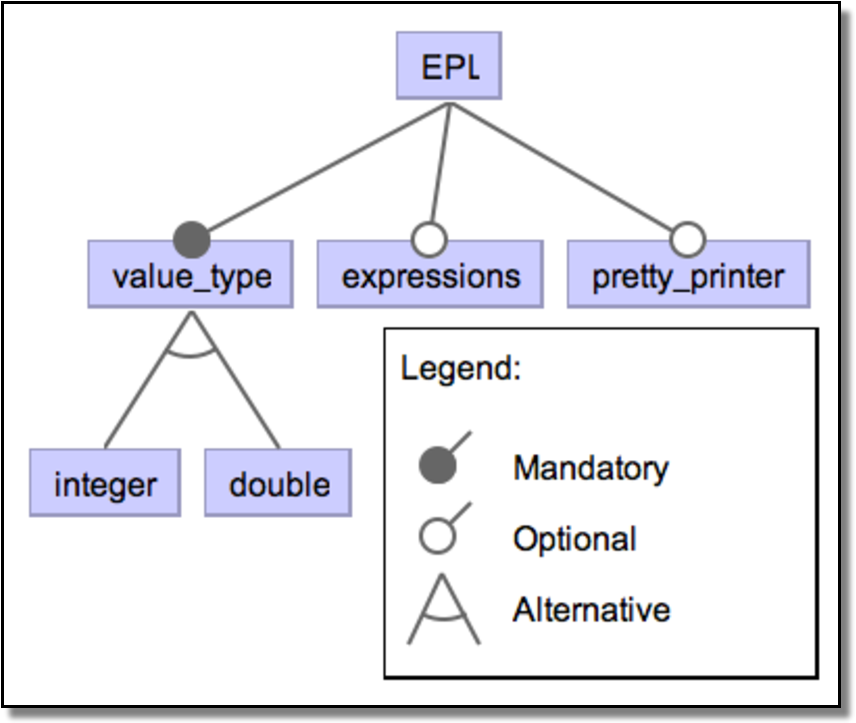
\includegraphics[scale=0.35]{doc/images/epl_fm}
\label{fig:epl_fm}
\caption{EPL feature model} 
\end{wrapfigure} 


In this section we illustrate the use of FOP through an AHEAD implementation 
of a slight adaptation of the Expression Product Line (EPL)~\cite{}---Figure~\ref{fig:epl_fm} shows 
the EPL feature model. Regarding our design decisions, 
in this case we implemented the mandatory features using a \textsc{base} AHEAD package (Figure~\ref{fig:epl-base}), which
declares a class hierarchy involving an interface (\texttt{Expression}) and
several classes (\texttt{Value}, \texttt{BinaryExpression}, \texttt{AddExpression}, and 
\texttt{SubExpression}), and one AHEAD package for each non-mandatory feature (see Figure~\ref{fig:epl-features}). Note 
that an AHEAD package contains eihter (a) plain Java entities (class or interface) declarations or (b) 
Java entities refinements. A refinement 
might override methods declared in other packages or 
introduce new attributes or methods in existing classes 
or interfaces. In this simple example, we do not implement any 
method overriding through class refinements---the refinements 
only introduce new elements to the \textsc{Base} AHEAD package 
of Figure~\ref{fig:epl-base}.  

\begin{figure}[htb]
\centering{
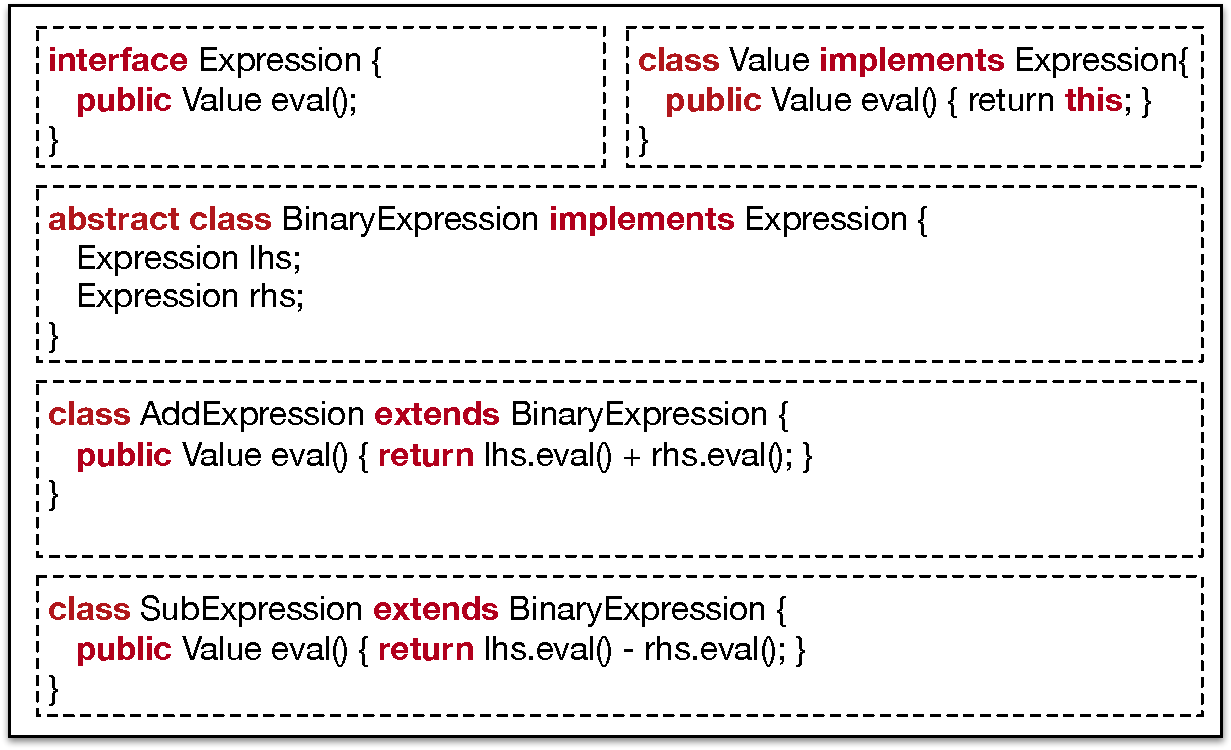
\includegraphics[scale=0.5]{doc/images/base.pdf}
}
\label{fig:epl-base}
\caption{The \textsc{base} package of the Expression Product Line}
\end{figure} 

The details of the EPL AHEAD non-mandatory feature packages are as follows. 

\begin{itemize}
\item Features \texttt{integer} and {double} refine the \texttt{Value} class of 
the \textsc{Base} package by introducing a new attribute named 
\texttt{value}, either with type \texttt{int} or \texttt{double}. According 
to the EPL feature model, only one of these features might be selected for 
a given product. 

\item The \texttt{expressions} feature introduces two new expressions 
to those declared in the \textsc{Base} package, one for multiplication 
and another for division. This particular feature does not refine 
existing classes, only introduces new ones. 

\item The \texttt{pretty\_printer} feature introduces the support for 
\emph{pretty printing} expressions. It refines the \texttt{Expression} 
interface and the \texttt{BinaryExpression} and \texttt{Value} classes, 
introducing a new method \texttt{print()} and also a 
new attribute (\texttt{operator}) for the \texttt{BinaryExpression} class.

\end{itemize}


\begin{figure}[htb]
\centering{
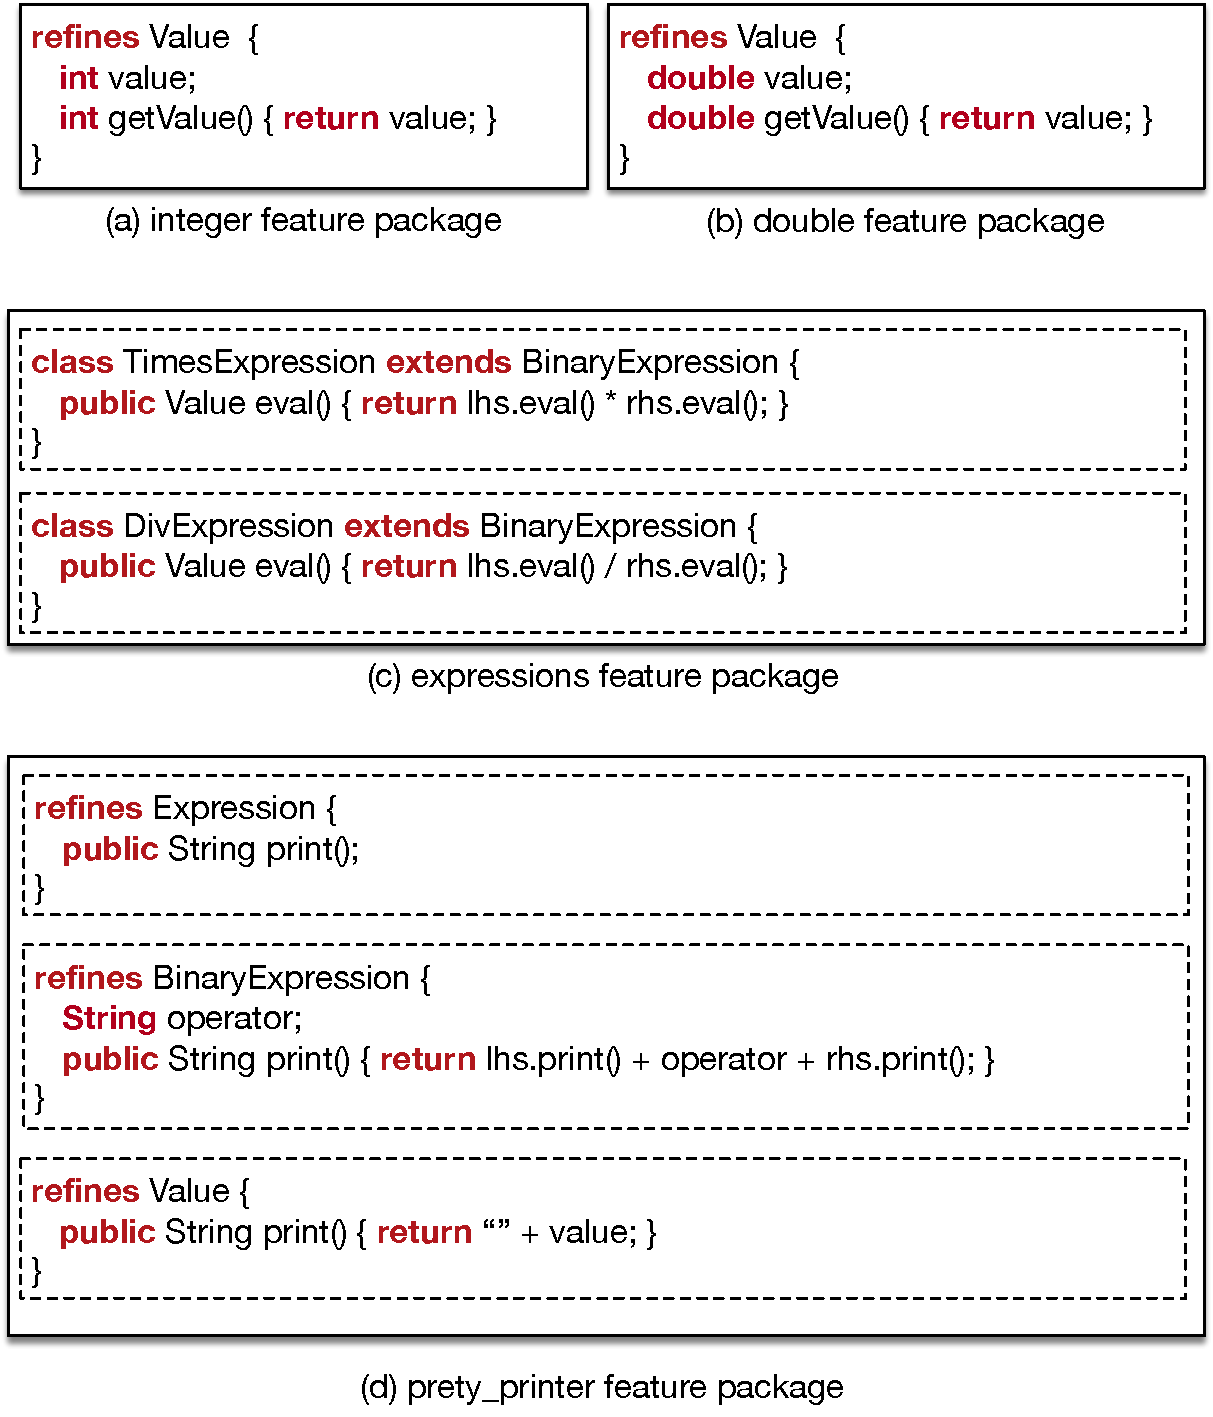
\includegraphics[scale=0.5]{doc/images/features.pdf}
}
\label{fig:epl-features}
\caption{Non-mandatory feature implementations of the Expression Product Line}
\end{figure} 

In the case we generate a product with  
a feature selection consisting of 
\texttt{EPL}, \texttt{value\_type(double)}, 
and \texttt{pretty\_printer}, we will get 
a product as shown in Figure~\ref{fig:epl-instance}. 



